\begin{tikzpicture}
	\node (A) at (-2.5,-3.5) {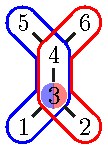
\includegraphics[scale=.8]{pathIntersectionClosedA}};
	\node (B) at (2.5,-3.5) {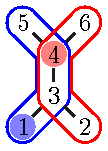
\includegraphics[scale=.8]{pathIntersectionClosedB}};
	\node (C) at (-2.5,3.5) {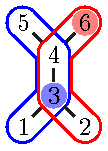
\includegraphics[scale=.8]{pathIntersectionClosedC}};
	\node (D) at (2.5,3.5) {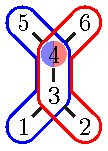
\includegraphics[scale=.8]{pathIntersectionClosedD}};
	\node (EF) at (1.15,0) {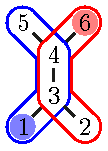
\includegraphics[scale=.8]{pathIntersectionClosedEF}};
	\node (EF) at (-1.15,0) {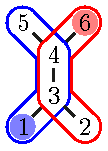
\includegraphics[scale=.8]{pathIntersectionClosedEF}};
	\node (piA) at (-2.5,-2.3) {$314625$};
	\node (piB) at (2.5,-2.3) {$146325$};
	\node (piC) at (-2.5,2.3) {$631425$};
	\node (piD) at (2.5,2.3) {$463125$};
	\node (piE) at (1.2,1.2) {$164325$};
	\node (piF) at (-1.2,-1.2) {$163425$};
	\node[draw,circle,inner sep=1] at (-3.2,-3.5) {$A$};
	\node[draw,circle,inner sep=1] at (3.2,-3.5) {$B$};
	\node[draw,circle,inner sep=1] at (-3.2,3.5) {$C$};
	\node[draw,circle,inner sep=1] at (3.2,3.5) {$D$};
	\node[draw,circle,inner sep=1] at (.5,0) {$E$};
	\node[draw,circle,inner sep=1] at (-.5,0) {$F$};
	\node at (0,0) {$=$};
	\draw (piA.north) -- (piC.south);
	\draw (piA.east) edge [out=0, in=180, looseness=1.5] (piD.west);
	\draw (piB.north) -- (piD.south);
	\draw (piB.north) edge [out=90, in=0, looseness=.5] (piE.east);
	\draw (piF.west) edge [out=180, in=270, looseness=.5]  (piC.south);
	\draw (piF.east) edge [out=0, in=180, looseness=.7] (piE.west);
\end{tikzpicture}
